%------------------------------------------------------------------
%
% Vorlage für Abschlussarbeiten an der Technischen Hochschule Ingolstadt
% Bachelorarbeit/Masterarbeit
%
% Angepasst auf Seminararbeit
%
% V1 05.12.2011		Dr. Paul Spannaus
% V2 07.07.2012		Dr. Paul Spannaus
% V3 10.03.2013		Dr. Paul Spannaus
% V4 28.01.2014		Dr. Paul Spannaus
% V5 31.10.2014 	Dominik Schlecht
% 	
% -----------------------------------------------------------------
% -----------------------------------------------------------------

\documentclass[a4paper,11pt,DIV=11,BROC=5mm,bigheadings,idxtotoc,cleardoubleempty,halfparskip,oneside,openright]{scrreprt} % 

%Packages
\input{configs/packages}

%%-------------Silbentrennung--------------------------------------
\hyphenation{}

%Nomenklatur
% z.B. (1)  \nomenclature{$v_0$}{Startgeschwindigkeit}   -> Formelverzeichnis
\nomenclature[A]{USB}{Universal Serial Bus}

%%-------------Index-----------------------------------------------
\makeindex
\makenomenclature

%------------------------------------------------------------------
% Angabe der zu verwendenden Dateien, sodass nur z.B. das aktuelle 
% Dokument compiliert wird; den Rest mit % auskommentieren
\includeonly{
	chapter/title_page,
	chapter/thanks_statement,
    chapter/einleitung,
    chapter/szenario,
    chapter/USB,
    chapter/policie,
    chapter/UmgehenUSBPolicies,
    chapter/FazitGegenmassnahmen,
	chapter/appendix
}


%------------------------------------------------------------------------

%-----------------------------------------------------------------
%---------------Dokumentenbeginn----------------------------------
%-----------------------------------------------------------------
\begin{document}
			
	
% Titelseite
\begin{titlepage}

\phantom{tmpText}

\vspace{1cm}

\begin{figure}[h!]
\centering
\includegraphics[width=\textwidth]{bilder/thi_logo_cropped.pdf}
\end{figure}

  \begin{center}

%\vspace{1cm}
    
    
    \textbf{{\large Seminararbeit/Whitepaper} \\[3ex]
    {\LARGE Umgehen von PID und VID basierten USB-Policies} \\[1ex]
    %
    \vfill
    %
    angefertigt von \\
    Dominik Schlecht \\[2ex] %Vorname Nachname
    %
    \vfill
    %
    Betreuer:} \\%[5ex]
    \begin{tabular}{ll}
      Technische Hochschule Ingolstadt: & Dr. Stanislaus \\
      Allianz Deutschland AG: & Dr. Stremmel und Herr Gerhager
    \end{tabular} \\[2ex]
    %
    \vfill
    %
    Ingolstadt, \today
  \end{center}
\end{titlepage}
		

	
%------------------------------------------------------------------------

% Nummerierung
\pagenumbering{roman}

% Sperrvermerk
\chapter*{Sperrvermerk}
Die vorliegende Arbeit \glqq Umgehen von USB-Deskriptor basierten USB-Policies am Beispiel einer virtuellen Umgebung\grqq\ wurde mit Unterstützung der Allianz Deutschland AG erstellt. Es sind jedoch keine internen, vertraulichen oder streng vertraulichen Informationen enthalten. Die Weitergabe des Inhalts der Arbeit im Gesamten oder in Teilen sowie das Anfertigen von Kopien oder Abschriften -- auch in digitaler Form -- sind grunds\"{a}tzlich erlaubt.
\addcontentsline{toc}{chapter}{Sperrvermerk}

% Erkl\"{a}rung
\chapter*{Erkl\"{a}rung}
Hiermit erkl\"{a}re ich, dass ich die vorliegende Seminararbeit bis auf die offizielle Betreuung durch den Aufgabensteller selbstst\"{a}ndig und ohne fremde Hilfe verfasst habe.\par
Die verwendeten Quellen sowie die verwendeten Hilfsmittel sind vollst\"{a}ndig angegeben. W\"{o}rtlich \"{u}bernommene Textteile und \"{u}bernommene Bilder und Zeichnungen sind in jedem Einzelfall kenntlich gemacht. \\[10ex]
Ingolstadt, \today
\addcontentsline{toc}{chapter}{Erkl\"{a}rung}

% Danksagung (optional)
\chapter*{Danksagung}
An dieser Stelle möchte ich mich bei allen Bedanken, die mich bei der Erstellung dieser Arbeit unterstützt haben. Besonderer Dank dabei gebührt den Kollegen aus der Allianz Deutschland AG und meinen Eltern.

\begin{flushright}
\sffamily Dominik Schlecht, \today
\end{flushright}
\addcontentsline{toc}{chapter}{Danksagung}


%------------------------------------------------------------------------

		\cleardoublepage	
					
			% Inhaltsverzeichnis
			%\setcounter{\secnumdepth}{2} % Zwei Ebenen im Inhaltsverzeichnis auflisten
			\tableofcontents
				\cleardoublepage	
		
			% Abkrzungsverzeichnis
			\printnomenclature
				\cleardoublepage	
			
%------------------------------------------------------------------------
			% Neunummerierung des Hauptteils
			\pagenumbering{arabic}
			\setcounter{page}{1}            
            \cleardoublepage
            
            \chapter{Einleitung}
In Zeiten von Heartbleed und Shellshock, Snowden und der NSA und der fortlaufenden Digitalisierung der Industrie und Gesellschaft wird das Thema Informationssicherheit immer wichtiger. Daten werden, unabhängig davon, ob diese Privatpersonen oder Firmen zugeordnet sind, immer wertvoller. So ergeben sich Beispielsweise aus einem gehackten Smartphone einer Privatperson Informationen wie E-Mail-Adressen, Kontakten und Chatverläufen bis hin zu Passwörter für das Online-Banking oder persönlichen Bildern. Da diese Informationen auf dem Schwarzmarkt oft zu nicht zu vernachlässigenden Preisen gehandelt werden, hat sich hier ein neuer Markt entwickelt. Black-Hat-Hacker oder Gruppen versuchen über Phishing-Mails oder Virenkampagnen so viele Daten wie Möglich zu sammeln, um diese im Anschluss zu verkaufen. Diese Tätigkeiten werden oft unter dem Schlagwort Cybercrime zusammengefasst. Umso kritischer in Hinsicht auf den möglichen finanziellen Schaden ist Cybercrime jedoch, wenn es um Unternehmen geht. Würde als Beispiel die Webseite eines Versandunternehmens von Hackern offline genommen werden, entstehen reale Verluste, da die Käufer auf andere Shops wechseln. Ähnlich kritisch wäre es, wenn streng vertrauliche Dokumente von Unternehmen, wie z.B. Konstruktionsskizzen oder Quellcode, durch Hacker erbeutet und an ein Konkurrenzunternehmen verkauft würden. So schätzt die Firma McAffee im Jahr 2014 den Verlust für die Wirtschaft durch "Cybercrime" auf bis zu 575 Milliarden USD\footnote{Siehe: $http://csis.org/files/attachments/140609\_McAfee\_PDF.pdf$}. 
Um diesem Trend entgegen zu wirken, müssen Unternehmen Maßnahmen ergreifen, welche das Schutzniveau erhöhen. Oft wird hier nur auf die technische Seite geachtet, z.B. auf das schnelle Patching von Servern. Dies ist sicherlich ein essentielle Bestandteil, oft wird jedoch die menschliche Komponente vernachlässigt, obwohl Social Engineering wohl zu den häufigsten Angriff Szenarien zählt. Dabei ist dies oft der erste Einfallspunkt für Cyberkriminelle. Für professionelle Hacker ist es kein Problem, eine E-Mail mit gefälschtem Absender und einem noch nicht erkannten Virus im Anhang zu verschicken. Öffnet der Mitarbeiter der Firma, welcher eine solche E-Mail empfängt, den Anhang ergeben sich gute Chancen für den Hacker Zugriff in das interne Netzwerk der Firma zu erlangen. Um dieses Risiko zu minimieren werden bei der Allianz Deutschland AG, im weiteren Verlauf AZD genannt, Awareness-Kampagnen mit Postern und Hinweistafeln, jedoch auch Schulungen mit Themen wie Spam und Phishing, organisiert. Diese Vorträge werden von wechselnden Mitarbeitern der Sicherheitsabteilung gehalten, welche im vorhinein Folien mit PowerPoint entwerfen und Demonstration entwickeln, an welchen das Themengebiet den Zuhörern praxisnah erläutern werden kann. Findet dieses ohne ein zentrales Programm statt, ergeben sich Problemfelder wie der Austausch, die Aktualität oder der Qualität der Vortragsmaterialien. Bei diesen und anderen Problemen soll das Security Awareness Framework, kurz SAF, Abhilfe schaffen.
\\
\\
\\
$[TODO ->]$Diese sind dann oft veraltet oder instabil. Zudem werden die Demos oft unter den Kollegen der Sicherheitsabteilungen nicht ausgetauscht. Dies hat mehrere Gründe, angefangen davon, dass diese oft nur für den Ersteller verständlich sind bis hin zu technischen Problemen wie der Größe oder dem Format der Virtuellen Maschine, auf welchen die Demos oft gespeichert sind. Diese Probleme soll durch das Security Awareness Framework gelöst werden.
                \cleardoublepage
                
			\chapter{Szenario}
Bei einer Prüfung interner Regularien bei der Informationssicherheit wurde das Thema USB-Geräte in Verbindung mit Thin oder auch sogenannten Zero-Clients aufgegriffen. Hier soll aus gegeben fachlichen Anlässen eine Möglichkeit geschaffen werden, lokale USB-Geräte, wie z.B. USB-Sticks oder USB-CD-Laufwerke an die virtuelle Maschine des Benutzers weiter zu leiten. Hier galt es, das Risiko zu prüfen und entsprechende Gegenmaßnahmen zu entwickeln. 
Würde man das Durchstellen von USB-Geräten im Allgemeinen erlauben, so würden sich erhebliche Gefahren ergeben, welche unter \ref{GefBeiUSB} erläutert werden. Um dem vorzubeugen, soll auf Basis einer Policy, welche in \ref{Policies} weiter erläutert wird, das Durchstellen auf bestimmte Geräte begrenzt werden. Dies geschieht bei dem hier getesteten Produkt über die Filterung nach USB-Deskriptoren wie \textit{idVendor} und \textit{idProduct}, welche ein USB-Device, z.B. einen bestimmten USB-Stick oder ein USB-CD-Laufwerk, eindeutig identifizieren sollen. Diese Felder werden unter \ref{Deskriptoren} weiter erläutert.
Bei der durchgeführten Sicherheitsprüfung stellte sich jedoch heraus, dass USB-Deskriptoren keinen Sicherungen unterliegen und somit mit Hilfe bestimmter Geräte gezielt Emuliert werden können. Diese Umgehung der Policy soll in diesem Dokument erläutert und aufgezeigt werden. Den Proof-Of-Concept finden Sie unter \ref{PoC}.

\begin{figure}[htbp]
\begin{tikzpicture}[
	scale=1,
	line width=0.25mm,
	every node/.style={
		scale=1, 
		text=THIblue},
	align=center,
	node distance=4cm,
	comp/.style={
		fill=white,
		rectangle,
		draw,
		minimum size=2.5cm},
	driver/.style={
		fill=white,
		rectangle,
		draw,
		yshift=2cm,
		xshift=-1cm},
	device/.style={
		fill=white,
		rectangle,
		draw},
	policie/.style={
		fill=white,
		rectangle,
		draw,
		yshift=-2cm,
		xshift=-1.5cm}
	]
	
	\node[comp] (thinclient) at (0,0){Thinclient};
	\node[driver] (thinclientUSB) [below right of=thinclient] {USB-Treiber};
	\node[device] (USBDevice) [right of=thinclientUSB, xshift=-1cm] {USB-Device};

	\node[comp] (hypervisor) [above of=thinclient] {Hypervisor};
	\node[driver] (hypervisorUSB) [below right of=hypervisor] {USB-Treiber};
	\node[policie] (hypervisorPol) [above right of=hypervisor] {Policie};
	
	\node[comp] (VM) [above of=hypervisor] {VM};
	\node[driver] (VMUSB) [below right of=VM] {USB-Treiber};
	\node[policie] (VMPol) [above right of=VM] {Policie};
		
	\draw[->]
		(USBDevice) --
			node[above]{1.}
				(thinclientUSB);	
	
	\draw[<->]
		(thinclientUSB) -- 
			node[right]{2.}
				++(0,-1) -| (USBDevice);
	
	\draw[->]
		(thinclient.125) -- 
			node[left]{3.}
				(hypervisor.235);
	
	\draw[<->]
		(hypervisor.10) -- 
			node[above]{4.}
				++(2.5,0) |- (hypervisorPol);
	
	\draw[->]
		(hypervisor.270) -- 
			node[left]{5.}
				(thinclient.90);
				
	\draw[->]
		(thinclient.55) -- 
			node[left]{6.}
				++(0,1.25)-|(hypervisorUSB);
	
	\draw[->]
		(hypervisor) --
			node[left]{7.}
				++(0,2.5)-|(VMUSB);
	
	\draw[<->]
		(VM.10) --
			node[above]{8.}
				++(2.5,0) |- (VMPol);
	
\end{tikzpicture}
\caption{Ablaufübersicht}
\label{fig:Ablauf}
\end{figure}

\begin{description}
	\item[Schritt 1: ] Ein USB-Gerät wird angesteckt.
	\item[Schritt 2: ] Der USB-Treiber des Thinclients bindet das Gerät ein. TODO Prüfen was übertragen wird
	\item[Schritt 3: ] Der Thinclient leitet entsprechende Deskriptor-Felder an den Hypervisor weiter.
	\item[Schritt 4: ] Der Hypervisor prüft die Deskriptor-Felder gegen die Hypervisor-Policy. Diese erlaubt entweder das Durchstellen oder verbietet es. Wird die Durchstellung verboten, wird der USB-Stick nicht an die Hypervisor-Umgebung weitergeleitet und damit würde der Ablauf enden. Im Folgenden wird angenommen, dass der USB-Stick weitergeleitet wird.
	\item[Schritt 5\&6: ] Der Hypervisor fordert den USB-Stick beim Thinclient an und bindet diesen ein.
	\item[Schritt 7: ] Der Hypervisor gibt das USB-Device an die VM weiter.
	\item[Schritt 8: ] Die VM prüft das USB-Device anhand der Deskriptor-Felder gegen die VM-Policy und bindet diesen entweder ein oder lehnt diesen ab.
\end{description}

			\chapter{USB}
USB ist eine Schnittstelle, welche so gut wie alle mordernen Rechner bsitzten. Es ist unter anderem Möglich darüber Geräte wie Kopfhörer, Joysticks aber auch Wechseldatenträger an zu schließen. Im letzteren Bereich ersetzt USB die bisher vorherschende CD/DVD-Technologier, da auf einem USB Stick mehr Daten in höherer Geschwindigkeit gespeichert werden können.
\section{Gefahren bei USB}\label{GefBeiUSB}
USB-Geräte stellen Gefahren auf verschiedenen Ebenen dar. Zum einen werden USB-Sticks, zumindest in dem Szenario, das hier betrachtet wurde, von Dritten an Mitarbeiter gegeben. Das heist, dass der Dritte, insofern dieser die nötige kriminielle Energie aufweist, ein prepariertes Gerät einschicken könnte. Erschwerend kommt hinzu, dass der Mitarbeiter keine Möglichkeit hat, ein böses USB-Gerät von einem normalen zu unterscheiden. Auch besteht die Möglichkeit für den Dritten den Angriff über längerere Zeit vorzubereiten, da kein Zeitdruck besteht, im Gegenteil, USB-Geräte sind gerade noch im Aufwärtstrend. TODO CD vs USB Statistik. Bei der Manipulation sind verschiedene Szenarien denkbar. Einige sind in den nächsten Sektionen aufgeführt.

\subsection{Viren}
Viren sind eine wachsende Bedrohung in der heutigen Zeit. Vor einigen Jahren waren einige wenige Virenfamilien weit verbreitet. So konnten Virenhersteller über signaturbasierte Suchalgorithmen nach bekannten Mustern suchen und Viren identifizieren. In den letzten Jahren zeichnet sich jedoch der Trend ab, dass Viren sich schneller weiterentwickeln und zudem oft polymorph programmiert sind, also ihr aussehen bei einer Infektion verändern. Dadurch werden signaturbasierte Erkennungen immer uneffizienter und die Gefahr, dass ein Rechner unerkannt Infiziert wird, steigt. Eine Infektion passiert zumeist über sogenannte Browserexploits, also preparierte Webseiten, welche Lücken in der Software des Users nutzten, oder durch E-Mails verbreitet. In dem von uns betrachteten Szenario würde ein krimineller Dritter oder aber auch ein unwissinder Dritter, dessen Rechner von einem Virus infiziert ist, einen USB-Stick mit einem Virus einschicken. Dabei wird im folgenden zwischen Trojaner, welche sich auf der Treiberebene einnissten, unterschieden.

\subsubsection{Viren auf Dateiebene}
Ein Trojaner ist eine Programm, welches sich als normale Software tarnt aber Schadcodefunktionalität mitliefert. \cite{Stamp2006} Will ein Benutzer das vermeitlich sinnvolle Programm installieren, wird im Hintergrund unbemerkt die Schadroutine mitinstalliert und gestartet. Dieser Schadecode hat oftmals Funktionalitäten wie Keylogger, Backdoors oder ein herkömmliches Rootkit. Auf unser Szenario übertragen müsste ein Benutzer also einen USB-Stick einstecken und ein darauf befindliches Programm starten. Ist der Virus bereits bekannt, könnte Virenscanner diesen finden un blockieren, jedoch ist es Aufgrund des Fortschritts immer öfter der Fall, dass Viren sich trotz gleicher Funktionaliät ihr aussehn veränder und dadruch von den Pattern des Virenschutzes nicht mehr erfasst werden.
			
\subsubsection{Viren auf Treiberebene}
Schwieriger zu entdecken sind Viren auf Treiberebene. Diese Nutzen lücken in der Firmware der im Computer verbauten Hardware und infizieren diese. So zeigte Karsten Nohl TODO Quelle zuletzt einen Angriff, in welchem er einen USB-Stick so manipuliert, dass dieser bei Kontakt mit einem Computer einen entsprechenden Trojaner ausführt. Dieser Trojaner war jedoch wiederrum in der Lange, andere USB-Stickts zu infizieren.

\subsection{Dateneinschleußung}

			
\subsection{Datenabfluss}
Neben den Gefahren von außen müssen jedoch auch sogenannte \glqq Inside-Threaths\grqq beachtet werden. Dies wären Mitarbeiter, welche z.B. interne IT-Systeme manipulieren, um sich Vorteile oder Reichtümer zu verschaffen. Das wohl bekannteste Beispiel wäre hier wohl ein TODO Kevin Midnick Geschichte. Bezogen auf USB wäre ein Risiko der Abfluss von Daten, also wenn ein Mitarbeiter Daten auf einem USB-Stick speichert und diese mit nach Hause nimmt, um diese zu Verkaufen oder sich zu bereichern. Denkbar wären zum Beispiel Kundendaten, bei Admins Passwörter, Geschäftsberichte oder sonstige Unternehmensgeheimnisse. Diese können oft für Geld in einschlägigen Bereichen des Internets verkauft oder bei Geschäftsberichten zur Manipulation am Finanzmarkt genutzt werden. Auch wäre eine Abwerbung eines Mitarbeiters von einem anderen Unternehmen für Industriespionage denkbar.
Eine neue Bedrohung sind Geheimdienste, welche Personen in eine Unternehmen einschleußen oder Mitarbeiter abwerben, um Daten übe die Kunden zu sammeln. Dies wurde erst letztens durch von Edward Snowden veröffentlichte Dokumente publik. TODO Quelle

\section{Technische Ablauf beim Einstecken eines USB-Devices}
Einstecken => Felder werden übertragen => Windows sucht nach Treiber und installiert diese

\section{Descriptoren}
Der USB-Specifikation, welche von dem USB Implementers Forum, Inc.\footnote{http://www.usb.org/about} festgelegt wird, sieht Felder vor, welche Informationen zu dem Gerät beinhalten.
\begin{wrapfigure}{l}{0pt}%{0.5\textwidth}
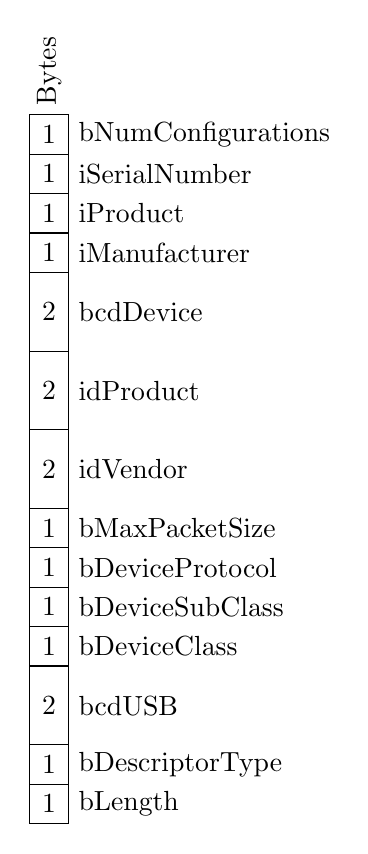
\begin{tikzpicture}[scale=1]
	\draw (0,0) rectangle (0.5,0.5);
	\draw (0.25, 0.25) node {1};
	\draw (0.5, 0.25) node[right]{bLength};
	
	\draw (0,0.5) rectangle (0.5,0.5);
	\draw (0.25, 0.75) node {1};
	\draw (0.5, 0.75) node[right]{bDescriptorType};
	
	\draw (0,1) rectangle (0.5,1);
	\draw (0.25,1.5) node {2};
	\draw (0.5,1.5) node[right]{bcdUSB};
	
	\draw (0,2) rectangle (0.5,0.5);
	\draw (0.25,2.25) node {1};
	\draw (0.5,2.25) node[right]{bDeviceClass};

	\draw (0,2.5) rectangle (0.5,0.5);
	\draw (0.25,2.75) node {1};
	\draw (0.5,2.75) node[right]{bDeviceSubClass};

	\draw (0,3) rectangle (0.5,0.5);
	\draw (0.25,3.25) node {1};
	\draw (0.5,3.25) node[right]{bDeviceProtocol};

	\draw (0,3.5) rectangle (0.5,0.5);
	\draw (0.25,3.75) node {1};
	\draw (0.5,3.75) node[right]{bMaxPacketSize};
	
	\draw (0,4) rectangle (0.5,1);
	\draw (0.25,4.5) node {2};
	\draw (0.5,4.5) node[right]{idVendor};
	
	\draw (0,5) rectangle (0.5,1);
	\draw (0.25,5.5) node {2};
	\draw (0.5,5.5) node[right]{idProduct};
	
	\draw (0,6) rectangle (0.5,1);
	\draw (0.25,6.5) node {2};
	\draw (0.5,6.5) node[right]{bcdDevice};
	
	\draw (0,7) rectangle (0.5,0.5);
	\draw (0.25,7.25) node {1};
	\draw (0.5,7.25) node[right]{iManufacturer};
	
	\draw (0,7.5) rectangle (0.5,0.5);
	\draw (0.25,7.75) node {1};
	\draw (0.5,7.75) node[right]{iProduct};
	
	\draw (0,8) rectangle (0.5,0.5);
	\draw (0.25,8.25) node {1};
	\draw (0.5,8.25) node[right]{iSerialNumber};
	
	
	\draw (0,8.5) rectangle (0.5,0.5);
	\draw (0.25,8.75) node {1};
	\draw (0.5,8.75) node[right]{bNumConfigurations};
	
	\draw (0,9) rectangle (0.5,0.5);
	
	\draw (0.25, 9) node[rotate=90, right] {Bytes};
\end{tikzpicture}
\caption{USB-Felder}
\end{wrapfigure}

Dies Umfasst die technische Informationen wie die Länge der gesamten Felder im \glqq bLength\grqq-Feld oder das Protokoll des Geräts im \glqq bDeviceProtocoll\grqq-Feld über Informationen für das Betriebssystem wie \glqq idVendor\grqq, \glqq idProduct\grqq, \glqq bDeviceSubClass\grqq und \glqq bDeviceClass\grqq. Diese Felder mit der jeweiligen Länge sind in der Grafik dargestellt. Ein Feld hat dabei zwischen ein und zwei Bytes. Die Felder \glqq bDeviceClass\grqq, \glqq bDeviceSubClass\grqq, \glqq bDeviceProtocol\grqq sowie \glqq idVendor\grqq werden vom Herrsteller befüllt.\footnote{http://www.beyondlogic.org/usbnutshell/usb5.shtml} Das Betriebssystem nutzt die Felder meist um Treiber zu suchen oder auch das angeschlossene USB-Gerät gegen die Policie-Einstellungen zu prüfen. Um eigene Werte bei PID oder VID-Felder zu nutzten und damit sicher gestellt ist, dass nicht mehrere Herrsteller die selbe PID verwenden, müssen die Addressbereiche der PID bei dem USB Implementers Forum, Inc. gekauft werden. Dazu gibt es zwei Möglichkeiten. Man kann entweder ein Mitglied werden, wobei kosten von 5000 USD jährlich anfallen oder einmalig 5000 USD für einen Adressraum zahlen, man darf dann jedoch nicht das offizielle USB-Logo verwenden. \footnote{http://www.usb.org/developers/vendor/} Im folgenden werden die für dieses Dokument interessanten Felder weiter erläutert:

%\begin{figure}[h]
%	\setlength{\unitlength}{0.14in} % selecting unit length
%	\centering % used for centering Figure
%	\begin{picture}(36,10) % picture environment with the size (dimensions)
%% 32 length units wide, and 15 units high.
%		\put(0,4){BlaBLab}
%		\put(0,0){\framebox(2,3){1}}
%		\put(2,0){\framebox(2,3){1}}
%		\put(4,0){\framebox(4,3){1}}
%		\put(8,0){\framebox(2,3){1}}
%		\put(10,0){\framebox(2,3){1}}
%		\put(12,0){\framebox(2,3){1}}
%		\put(14,0){\framebox(2,3){1}}
%		\put(16,0){\framebox(4,3){1}}
%		\put(20,0){\framebox(4,3){1}}
%		\put(24,0){\framebox(4,3){1}}
%		\put(28,0){\framebox(2,3){1}}
%		\put(30,0){\framebox(2,3){1}}
%		\put(32,0){\framebox(2,3){1}}
%		\put(34,0){\framebox(2,3){1}}
%		\put(23,4){\framebox(6,3){$H_{C}(q)$}}
%		\put(0,5.5){\vector(1,0){3}}
%		\put(19.5,6.5) {$x_{C}(k)$}
%	\end{picture}
%	\caption{Aufbau der USB-Descriptoren}
%	% title of the Figure
%	\label{fig:lnlblock}
%	% label to refer figure in text
%\end{figure}			
$ $\\ \\ \\ \\ \\
\begin{description}
	\item[idVendor: ] Das idVendor-Feld wird von der USB Implementers Forum, Inc. festgelegt. Das Feld ist 2 Byte lang und ein Wert ist genau einem Herrsteller zugeordnet. Ersteht ein Unternehmen eine idVendor-Nummer, kann er über das idProduct-Feld frei verfügen.
	\item[idProduct: ] Das idProduct-Feld wird von einem Unternehmen vergeben, welches einen Wert im idVendor-Feld gekauft hat. Es ist ebenfalls 2 Byte lang. Damit könnte ein Unternehmen bis zu $2^{16}$ verschiedene Produkte beschreiben.
	
\end{description}
Das Feld PID steht für Produkt \glqq Identifier\grqq und beschreibt den Herrsteller des Geräts. TODO Tabelle
			
			
			\chapter{Richtlinien} \label{Policies}
Eine Policy ist ein Regelwerk, das die Rechte und Möglichkeiten von Benutzern auf einem IT-System beschreibt und eingrenzt. Es gibt verschiedene Arten von Policies. Im folgenden wird nur die beschrieben, die für den weiteren Verlauf der Arbeit relevant ist. Hier besteht eine Regel aus mehreren Bestandteilen, die entweder wahr oder falsch sind. Diese Bestandteile können per \textit{und}- oder \textit{oder}-Verknüpfungen zu einer Regel vereint werden.\\
Abstrakt ist eine Policy mit einem Regelwerk wie der Straßenverkehrsordnung zu vergleichen. Auch hier gibt es Vorgaben, wer, wann und wo fahren oder parken darf. So wird zum Beispiel bei einem Durchfahrtsverbot, das für Anlieger nicht gelten soll, folgende Regel festgelegt:
\begin{description}
	\item[Regel-1: ] Die Durchfahrt ist für alle verboten
	\item[Regel-2: ] \textit{oder} der Fahrer ist Anlieger.
\end{description}
Bezeichnen wir in dem Beispiel den Ausgang \textit{der Fahrer darf durch die Straße fahren} als \textit{1} und den Ausgang \textit{der Fahrer darf nicht durch die Straße fahren}, als \textit{0}, so wäre hier das Ergebnis
\begin{equation*}
	\alpha = Regel\text{-}1 \vee Regel\text{-}2
\end{equation*} mit 
\begin{equation*}
	Regel\text{-}1=0
\end{equation*}. Somit ergeben sich daraus für die verschiedenen Fälle von $Regel$-$2$
\[
	\alpha = 
		\begin{dcases*}
			0 & wenn Regel\text{-}1 gleich 0\\
			1 & wenn Regel\text{-}1 gleich 1
		\end{dcases*}
\]
. Ähnliche Regeln können über Policies auf Rechner festgelegt werden. Hier wäre eine mögliche vergleichbare Regel im Bezug auf Speicherzugriffe
\begin{enumerate}
	\item Der Zugriff auf diesen Ordner ist gesperrt
	\item außer der Benutzer hat die Kennung MaxMuster
\end{enumerate}
Solche Regeln werden jedoch nicht nur für die Organisation von Speicherzugriffen, sondern auch für das Sperren bestimmter Einstellungen oder mancher Geräte verwendet.


			\chapter{Umgehung der USB-Policies}\label{Angriff}

\section{Wie wird gefiltert}
Die in diesem Dokument benutzten USB-Policies werden über die USB-Deskriptoren \ref{Deskriptoren} definiert. Wollten wir etwa ein Gerät mit $idProduct=0x01$ und $idVendor=0x02$ freigeben aber alle sonstigen Geräte abweisen, so wäre folgende Regel möglich:
			\begin{itemize}
				\item Verbiete alle USB-Geräte
				\item Erlaube USB-Geräte mit
				\begin{itemize}
					\item $idProduct=0x01$
					\item $idVendor=0x02$
				\end{itemize}
			\end{itemize}
Die Regeln werden von oben nach unten gelesen, wobei spätere Regeln frühere überschreiben. Hier würden also zuerst alle USB-Geräte blockiert werden, außer das Gerät besitzt die $idProduct=0x01$ und $idVendor=0x02$. Dies scheint logisch, hat ein Gerät z.B. die $idProduct=0x03$, so tritt die \textit{Erlaube}-Regel nicht in Kraft und es bleibt die \textit{Verbiete}-Regel bestehen. Meldet sich ein Gerät mit $idProduct=0x01$ und $idVendor=0x02$ an, so gilt zwar auch zunächst die \textit{Verbiete}-Regel, jedoch trifft die \textit{Erlaube}-Regel zu und überschreibt die \textit{Verbiete}-Regel, sodass der Zugriff gewährt wird.
Diese Zugriffe können gegebenenfalls noch um eine \textit{Active-Directory-Gruppe} erweitert werden. Dies ist vor allem nützlich, wenn man nur bestimmten Benutzern die Möglichkeit geben will, auf USB-Geräte zu zu greifen. Wollten wir z.B. dem Benutzer \glqq Alice\grqq den Zugriff auf ein USB-Gerät mit der $idProduct=0x01$ und der $idVendor=0x02$ geben, so wäre die Regel:
			\begin{itemize}
				\item Verbiete alle USB-Geräte
				\item Ist $User=Alice$
				\item Erlaube USB-Geräte mit
				\begin{itemize}
					\item $idProduct=0x01$
					\item $idVendor=0x02$
				\end{itemize} 
			\end{itemize}

\section{Teensy}
Das Teensy ist ein Platine bestehend aus einem 72 MHz MK20DX256VLH7 Cortex-M4 Prozessor, 256 kbytes Flash Speicher und 64 kbytes RAM. Zudem verfügt es über eine USB-Schnittstelle. Man kann also ein Programm auf dem Teensy ablegen und dieses wird ausgeführt, wenn man den USB-Stick einsteckt. So kann man beliebige Signalfolgen über USB an ein anderes Gerät schicken.
			
\section{Concept}
Da die USB-Felder nicht durch Signaturen oder sonstige Möglichkeiten vor Manipulation geschützt sind, sollte es möglich sein, einen Teensy so zu programmieren, dass er sich als ein beliebiges Gerät ausgibt, also beliebige \textit{idProduct}- und \textit{idVendor}-Werte emuliert. Beschränkt eine USB-Policie den Zugriff auf ein bestimmtes Gerät, so könnte man dieses theoretisch mit dem Teensy nachahmen.
Um dies umzusetzen wurden verwendet:

\begin{itemize}
	\item Teensy 3.1 + USB-Kabel
	\item Arduino 1.0.5 (64bit) installiert unter \textit{$\sim$/teensy/arduino-1.0.5}
	\item Teensyduino 1.19 (64bit)
	\item Kali-Linux als Testbetriebssystem (64bit)
\end{itemize}

Zur Analyse, mit welchen idVendor und idProduct-Werten sich der Teensy meldet, wurde mit dem Kommando \glqq tail -f /var/log/syslog\grqq das zentrale Logfile des Linuxsystems ausgelesen. Beim ersten einstecken ergab sich dabei folgende Meldung:
\definecolor{gray}{rgb}{0.5, 0.5, 0.5}
\lstset{% general command to set parameter(s)
	basicstyle=\tiny\ttfamily,%\small, % print whole listing small
	keywordstyle=\color{THIblue}\bfseries\underbar,% underlined boldblack keywords
	identifierstyle=, % nothing happens
	commentstyle=\color{green}, % white comments
	stringstyle=\color{red}\ttfamily, % typewriter type for strings
	showstringspaces=false, % no special string spaces
	%numbers=left,
	%numberstyle=\color{gray},
	%numbersep=5pt,
	captionpos=b,
	breaklines=true}
	
% Define Language
\lstdefinelanguage{log}
{
  % list of keywords
  morekeywords={
    idVendor,
    idProduct
  },
  sensitive=false, % keywords are not case-sensitive
  %alsodigit={0482},
  morecomment=[l]{//}, % l is for line comment
  morecomment=[s]{/*}{*/}, % s is for start and end delimiter
  morestring=[b]" % defines that strings are enclosed in double quotes
}

\lstset{language=log}
\lstinputlisting[caption={tail -f syslog output},otherkeywords={=0482, 0482, =16c0, 16C0}]{documents/syslog.log}

Die wichtigen Werte, also die \textit{idVendor} gleich \textit{16c0} und die \textit{idProduct} gleich \textit{0482} sind farblich hervorgehoben. Nun bearbeitet man die usb-desc.h, welche die notwendigen Informationen bei einer Neubeschreibung des Teensy bereit hält. Der relevante Abschnitt sowie die zu ändernden Werte sind wieder farblich hinterlegt.

\lstset{language=C}
\lstinputlisting[caption={usb\_desc.h},linerange={112-130},language=c]{documents/usb_desc.h}

Ändert man hier die markierten Werte und beschreibt den Teensy mittels der Arduino-Software neu, so werden diese Deskriptoren verwendet. Das Programm ist dabei entbehrlich, hier wurde eine an den Teensy 3.1 angepasste Version des \textit{Blink}-Programms verwendet, welches im Anhang abgelegt ist. Kompiliert man das Programm nun und lädt es auf den Teensy, ergibt der \glqq tail -f /var/log/syslog\grqq -Befehl folgenden Output:

\lstset{language=log}
\lstinputlisting[caption={tail -f syslog output 2}, otherkeywords={=beef, BEEF}]{documents/syslog_2.log}

Wie man den farblich hervorgehoben Stellen sehen kann, meldet sich der Teensy nun mit geänderten Deskriptoren.

\section{Proof of Concept} \label{PoC}

			\chapter{Fazit und Gegenmaßnahmen}
Da der USB-Standard keine Möglichkeit bietet Geräte fehlerfrei, zum Beispiel über Signaturen, zu identifizieren, kann diese Ebene nicht als effektive Schutzmaßnahme einstufen und muss die Gefahren direkt eindämmen. Jedoch ist dies im Bezug auf die Exploits auf Treiberebene sehr schwer. Die einfachste und sicherste Methode wäre, die Benutzung von USB-Ports in einem Unternehmen per Richtlinie zu verbieten und die Ports eventuell sogar noch physikalisch zu versiegeln. Hier hätte man natürlich den Nachteil, dass USB-Geräte nicht mehr direkt genutzt werden könnten. Als Lösung für dieses Problem, könnte man eine Art Schleusen-System für USB-Geräte aufgebaut werden. So könnte man, wenn ein USB-Stick an die Firma geschickt wird, dieser in dem Terminal-Server eingebunden und die Daten an den gewünschten Empfänger weiterreicht werden. Die Vorteile sind hier, dass falls Viren auf dem USB-Stick enthalten sind, diese vorher am Terminalserver sowie bei der Netzwerkübertragung von mehreren verschiedenen Virenscanner überprüft sowie heuristischen Analysten unterworfen werden könnten. Ebenso würde bei einem manipulierten USB-Stick nicht der Rechner des Mitarbeiters sondern nur der Schleusen-PC infiziert. Trifft man hier entsprechende Sicherheitsmaßnahmen wie die Platzierung des Schleusen-PCs in der demilitarisierten Zone und einen regelmäßigen Tausch oder Neuinstallation des Schleusenrechners, kann man das Risiko relativ gering halten. Der Mitarbeiter würde in diesem Fall nur die Dateien bekommen und wäre von der Manipulation auf Treiberebene nicht betroffen. Zudem sind die im Vorfeld getroffenen Sicherheitsmaßnahmen für den Mitarbeiter transparent.
	
			
%------------------------------------------------------------------------
			
			% Anhang
			
%------------------------------------------------------------------------
% Anhänge
\appendix
\chapter{Appendix}
\section{Quellcode}

\lstset{% general command to set parameter(s)
	basicstyle=\small\ttfamily,%\small, % print whole listing small
	keywordstyle=\color{THIblue}\bfseries,% underlined boldblack keywords
	numbers=left,
	numberstyle=\color{gray},
	numbersep=5pt,
	captionpos=t}

\lstset{language=C}
\lstinputlisting[caption={Blink\_2.ino},language=c]{documents/Blink_2.ino}

\newpage
\section{Ergänzende Grafiken}

\begin{figure}[htbp]

\centering
\includegraphics[width=\textwidth]{bilder/EinstellungenArduino.png}
\label{fig:EinstellungenArduino}
\caption{Einstellungen Arduino}

\end{figure}

			
			% Literaturliste
			\newpage
			\bibliographystyle{plaindin}	% DIN Norm für Literaturdarstellung
			\bibliography{ref/ref_liste}	% Pfad und Datei der Ref-Datenbank
		
	\end{document}
%-----------------------------------------------------------------
